\section{Locomotion}

The walk used at RoboCup 2009 was a modified version of Aldebaran's walk that implemented pseudo omni-directional capabilities. Essentially, ALMotion was used to generate a set of predefined steps offline, the cached steps are then linked together online. This allowed the robot to walk on an arc of varying radius without stopping, and a \texttt{walkToPoint} interface was used to continuously specify the desired target after each behaviour iteration. However, in some instances the robot still needs to stop when changing directions, for example, to change from a forward walk to a sideways walk first requires the robot to stop.

A heuristic path planning algorithm was implemented to determine a fast way to get to a target point given the limited number of available steps. Paths consisting of permutations, with repetition, of the set of walk primitives (forward, arc, turn, backward and sideward) are trialled, the fastest permutation that goes through the desired target with the desired orientation is chosen. This process is repeated every time a new step is required, and the step which best implements the chosen path become the next step.

The source code for the walk engine is available as a standalone module at \href{http://github.com/soneoed/naowalkoptimiser}{http://github.com/soneoed/naowalkoptimiser}. The source release includes many things; the code to generate and cache the steps, the code for the walk engine itself, the scripted motion files for kicks, getups and saves, the fall-preservation control, and code used to optimise the joint stiffnesses as a function of gait cycle (along with the associated laser scanner robot tracking).

\subsection{Pattern Generation}

Aldebaran's ALMotion was used to generate walk primitives in the following directions; forward, arc, turn, backward and sideward. The arc primitive contains steps on arcs of radii from 5cm to 100cm in 5cm increments, and the turn primitive contains steps on turns of angle from 9 degrees to 180 degrees in 9 degree increments. The forward, backward and sideward only contain a single set of steps, in particular, only steps of a single length are possible while walking forwards or backwards, making lining up kicks difficult.

A walk primitive contains a set of steps. A set of steps includes steps for both left and right legs, and a start step, a second step, a normal step, and a stop step. If the walk primitive contains many directions, that is, a arc or turn walk primitive, there is a set of steps for each direction. Consequently, there are over 800 individual cached steps used by the walk engine, and they are organised as shown in Figure \ref{fig:LocomotionSteps}.

\begin{figure}[tbh]
	\begin{center}
		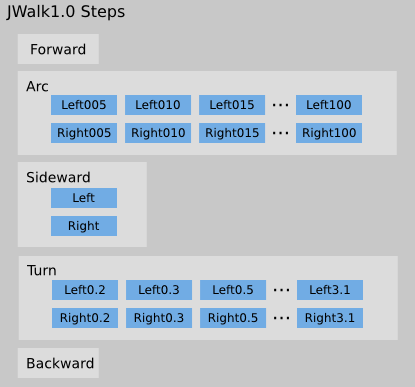
\includegraphics[width=0.6\textwidth]{locomotionfigs/steps.png}
		\caption{The organisation of cached steps used by the walk engine.}
		\label{fig:LocomotionSteps}
	\end{center}
\end{figure}

Each walk primitive has its own set of slightly different walk parameters, and in the case of arcs, a slightly different set of parameters was given based on the arc radius. The walk parameters are shown in Figure \ref{fig:LocomotionWalkParameters}.

\begin{figure}
	\begin{center}
		{\scriptsize\begin{verbatim}
		configureForwardWalk()
		   setWalkParameters(0.060, 0.012, 0.04, 0.5, 0.013, 0.007);
		   setWalkExtraParameters(4, -4, 0.23, 1.5);
		   setWalkGaitPeriod(23);
		   setWalkArmParameters(90*TO_RAD, 15*TO_RAD, 20*TO_RAD, 10*TO_RAD);

		configureBackwardWalk()
		   setWalkParameters(0.030, 0.012, 0.04, 0.5, 0.015, 0.012);
		   setWalkExtraParameters(4, -4, 0.23, 1.5);
		   setWalkGaitPeriod(24);
		   setWalkArmParameters(90*TO_RAD, 15*TO_RAD, 20*TO_RAD, 10*TO_RAD);

		configureArcWalk()
		   if (radius < 8)
		      setWalkParameters(0.030, 0.012, 0.04, 0.5, 0.013, 0.007);
		      setWalkGaitPeriod(22);
		   else if (radius < 12)
		      setWalkParameters(0.035, 0.012, 0.04, 0.5, 0.013, 0.007);
		      setWalkGaitPeriod(22);
		   else if (radius < 17)
		      setWalkParameters(0.040, 0.012, 0.04, 0.5, 0.013, 0.007);
		      setWalkGaitPeriod(22);
		   else if (radius < 42)
		      setWalkParameters(0.045, 0.012, 0.04, 0.5, 0.013, 0.007);
		      setWalkGaitPeriod(22);
		   else
		      setWalkParameters(0.065, 0.012, 0.04, 0.5, 0.013, 0.007);
		      setWalkGaitPeriod(24);
		   setWalkExtraParameters(4, -4, 0.23, 1.5);
		   setWalkArmParameters(90*TO_RAD, 15*TO_RAD, 20*TO_RAD, 10*TO_RAD);

		configureTurn()
		   setWalkParameters(0.060, 0.012, 0.04, 0.3, 0.01, 0.011);
		   setWalkExtraParameters(4, -4, 0.23, 1.5);
		   setWalkGaitPeriod(21);
		   setWalkArmParameters(90*TO_RAD, 15*TO_RAD, 20*TO_RAD, 10*TO_RAD);

		configureSideWalk()
		   setWalkParameters(0.060, 0.012, 0.04, 0.5, 0.00, 0.011);
		   setWalkExtraParameters(4, -4, 0.23, 1.5);
		   setWalkGaitPeriod(20);
		   setWalkArmParameters(90*TO_RAD, 15*TO_RAD, 20*TO_RAD, 10*TO_RAD);
		\end{verbatim}}
		\caption{The organisation of cached steps used by the walk engine.}
		\label{fig:LocomotionWalkParameters}
	\end{center}
\end{figure}

As with last year's walk engine \cite{JasonsAcraPaper} different joint stiffnesses were given to each joint, the stiffnesses were slightly updated for the new V3 NAO. The stiffnesses for every joint, except the two head joints, for each primitive are shown in Figure \ref{fig:LocomotionWalkParameters2}.

\begin{figure}
	\begin{center}
		{\scriptsize\begin{verbatim}
		forward =  [0.10, 0.25, 0.10, 0.25, 0.70, 0.26, 0.55, 0.25, 0.24, 0.28]
		backward = [0.10, 0.25, 0.10, 0.25, 0.70, 0.26, 0.55, 0.25, 0.23, 0.25]
		arc =      [0.10, 0.25, 0.10, 0.25, 0.70, 0.26, 0.55, 0.25, 0.23, 0.25]
		sideward = [0.10, 0.25, 0.10, 0.25, 0.70, 0.35, 0.55, 0.25, 0.23, 0.25]
		turn =     [0.10, 0.25, 0.10, 0.25, 0.70, 0.26, 0.55, 0.25, 0.23, 0.25]
		\end{verbatim}}
		\caption{The joint stiffnesses for each joint for each walk primitive used by the walk engine. The left arm and left leg stiffnesses are shown, but the same values are used for the right side.}
		\label{fig:LocomotionWalkParameters2}
	\end{center}
\end{figure}

\subsection{Step Linking}

The linking of steps to form a walk is simplified by having each walk primitive store each set of steps in a linked list. Basically the linked list is set up so that each step knows which step would follow if no direction change is required, and which step is required to bring the robot to rest. The rat's nest is shown in Figure \ref{LocomotionLinkedSteps}.

\begin{figure}[tbh]
	\begin{center}
		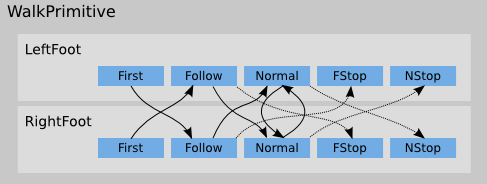
\includegraphics[width=0.6\textwidth]{locomotionfigs/linkedsteps.png}
		\caption{The organisation of a walk primitive used by the walk engine.}
		\label{LocomotionLinkedSteps}
	\end{center}
\end{figure}

A change in direction is essentially a transition from one walk primitive's linked list to the new direction's linked list, being careful to enter the new list at the correct point. There are several complications, the first is direction changes that first required the robot to stop. This is accomplished simply by selecting the appropriate stopping step, subsequent calls to walkToPoint will automatically select the first step in the new direction. The second complication is that many steps come in pairs, for example, walking on a rightward arc has a right and then a left step that must follow; calls for direction changes are ignored until the left step is completed. 

\subsection{Path Planning}

In order to maximise the utility of the walk engine given the limited number of available primitives a simple time-based heuristic path planning algorithm was implemented. Prior to the selection of every step the time taken by between 4 and 6 different candidate paths to reach the target position and orientation is calculated. The path with the shortest time is selected, and the next step is chosen to implement that path as closely as possible given the current pose of the robot.

The candidate paths consist of straight, arc, sideward, and turn segments.  In particular, for path planning with a final orientation, the candidate paths are arc-straight-arc, turn-straight-turn, turn-backward-turn and turn-sideward-turn, where the initial and final turn and arc segments may not be required. Figure \ref{fig:LocomotionPathPlanning} shows examples of the planned paths. Additionally, paths could be planned ignoring the final orientation.

\begin{figure}[tbh]
	\begin{center}
		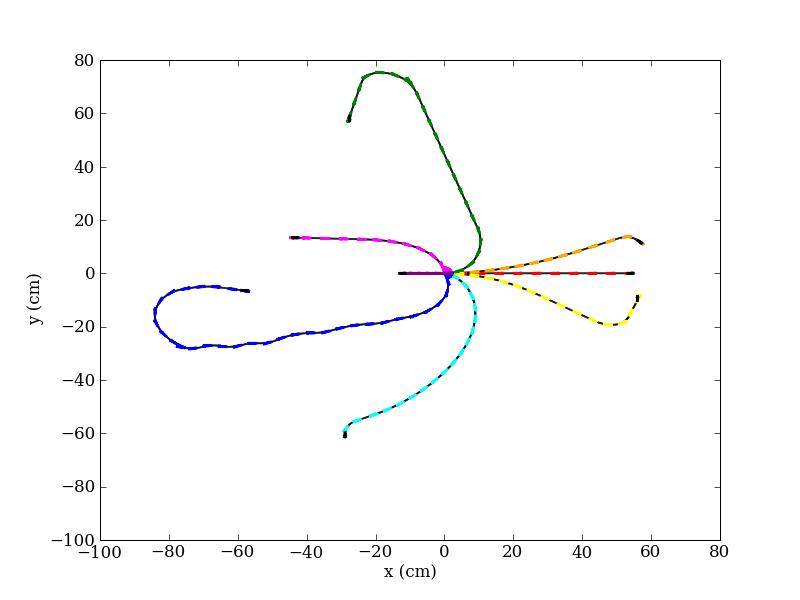
\includegraphics[width=0.8\textwidth]{locomotionfigs/pathplanning.png}
		\caption{A selection of planned paths for different target locations and orientations. The orientation and position of the simulated robot is shown with the coloured arrows for each path. The target location and orientation is shown with a black arrow.}
		\label{fig:LocomotionPathPlanning}
	\end{center}
\end{figure}

\subsection{Scripted Motion}
\subsubsection{Getups}
We have two getups; one for when it is lying on its chest, and another for when it is on its back. We found that Aldebaran's getup from front included with Choregraphe broke the HipYawPitch motor frequently. Consequently, we created a new one from scratch so that it was easier on this fragile joint. The motion also turned out to be slightly faster, but just as reliable. 

The getup from back was simply Aldebaran's script from Choregraphe.

\subsubsection{Kicks and Saves}
We have five kick scripts for each foot; two forwards, two sidewards and one backwards. The duplicate kicks target balls at different relative positions, for example, the two forward kicks are designed to kick balls close to the centre, and far from the centre. This was done to avoid need to line up kicks perfectly, especially given the limited walk engine.

We have three save scripts; a left save, a centre save and a right save. Each of the saves involves spreading the legs, for the left and right save the other foot remains on the ground making getting back up very easy. For the centre save both the left and right legs are spread, while the robot leans back on its arms,.

All of the script files for kicks and saves were generated using Aldebaran's Choregraphe. The motion script files, as a comma-separated file, are available at \href{http://github.com/soneoed/naowalkoptimiser}{http://github.com/soneoed/naowalkoptimiser}.

\subsubsection{Fall Protection Poses}
When the robot is falling over it goes into a fall protection pose to minimise damage to the robot. There are four protection poses; one for each falling direction. The forward pose attempt to have the robot land chest-first on the floor avoid damage to the arms and head, while the backward fall pose aims to have the robot land on its bottom in a sitting position again protecting the arms and head. The left and right fall poses tuck the left or right arm, respectively, into the narrow part of the torso. 
